\section{Introduction}

The estimation of directed and undirected graphs from high-dimensional data has received a lot of attention in the machine
learning and statistics literature \cite[e.g., see][and references therein]{buhlmann2011statistics}, due to
their importance in diverse applications including understanding of biological processes and disease mechanisms, financial
systems stability and social interactions, just to name a few \citep{sachs2005causal,wang2007local,sobel2000causal}. In the case of undirected graphs, the edges capture
conditional dependence relationships between the nodes, while for directed graphs they are used to model causal relationships \citep{buhlmann2011statistics}. 

However, in a number of applications the nodes can be {\em naturally partitioned} into sets that exhibit interactions both between
them and amongst them. As an example, consider an experiment where one has collected data for both genes and metabolites for
the same set of patient specimens. In this case, we have three types of interactions between genes and metabolites: regulatory interactions between the two of them and co-regulation within the gene and within the metabolic compartments. The latter two types of relationships can be expressed through undirected graphs within the sets of genes and metabolites, respectively, while
the regulation of metabolites by genes corresponds to directed edges. Note that in principle there are feedback mechanisms from the
metabolic compartment to the gene one, but these are difficult to detect and adequately estimate in the absence of carefully collected time course data. Another example comes from the area of financial economics, where one collects data on returns of financial assets (e.g. stocks, bonds) and also on key macroeconomic indicators (e.g. interest rate, prices indices, various
measures of money supply and various unemployment indices). Once again, over short time periods there is influence from
the economic variables to the returns (directed edges), while there are co-dependence relationships between the asset returns and the macroeconomic variables, respectively, that can be modeled as undirected edges.

Technically, such {\em layered} network structures correspond to multi-partite graphs that possess undirected edges and exhibit a 
directed acyclic graph structure between the layers, as depicted in Figure~\ref{fig:diagram}, where we use directed solid edges to denote the dependencies across layers and dashed undirected edges to denote within-layer conditional dependencies. 
%\usepackage{tikz}
\begin{figure}[h]
\centering
\caption{Diagram for a three-layered network}\vspace*{2mm}\label{fig:diagram}
\begin{boxedminipage}{9.2cm}
\def\layersep{3.5cm}
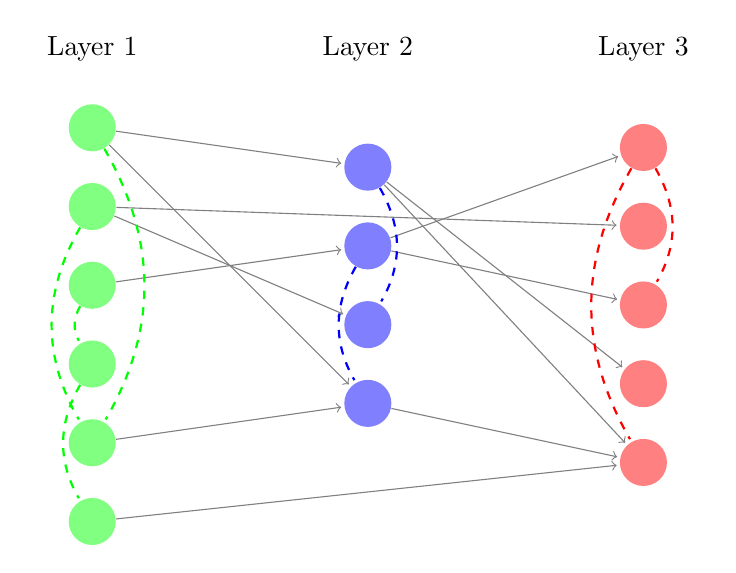
\begin{tikzpicture}[shorten >=1pt,->,draw=black!50, node distance=\layersep]
    \tikzstyle{every pin edge}=[<-,shorten <=1pt]
    \tikzstyle{neuron}=[circle,fill=black!25,minimum size=17pt,inner sep=0pt]
    \tikzstyle{input neuron}=[neuron, fill=green!50];
    \tikzstyle{output neuron}=[neuron, fill=red!50];
    \tikzstyle{hidden neuron}=[neuron, fill=blue!50];
    \tikzstyle{annot} = [text width=4em, text centered]

    % Draw the input layer nodes
    \foreach \name / \y in {1,...,6}
    % This is the same as writing \foreach \name / \y in {1/1,2/2,3/3,4/4}
        \node[input neuron] (I-\name) at (0,-\y) {};

    % Draw the hidden layer nodes
    \foreach \name / \y in {1,...,4}
        \path[yshift=-0.5cm]
            node[hidden neuron] (H-\name) at (\layersep,-\y cm) {};

    % Draw the output layer node
    \foreach \name / \y in {1,...,5} 
	   \path[yshift=-0.25cm]
		   node[output neuron] (O-\name) at (2*\layersep, -\y cm) {};
	    
    % % connect node in Layer 1 and Layer 2
    \path (I-1) edge (H-1); \path (I-1) edge (H-4);
    \path (I-2) edge (H-3);
    \path (I-5) edge (H-4);
    \path (I-3) edge (H-2);
    

    % Connect node in Layer 2 and Layer 3
    \path (H-2) edge (O-1); \path (H-2) edge (O-3);
    \path (H-1) edge (O-4); \path (H-1) edge (O-5);
    \path (H-4) edge (O-5);
    
    %  connect node in Layer 1 and Layer 3
    \path (I-2) edge (O-2); \path (I-6) edge (O-5);
    
    %  add within-layer connections
    \path[-,dashed, green,thick,bend left] (I-1) edge (I-5);
    \path[-,dashed, green,thick,bend right](I-2) edge (I-5);
	\path[-,dashed, green,thick,bend right](I-3) edge (I-4);
    \path[-,dashed, green,thick,bend right](I-4) edge (I-6);
    
    \path[-,dashed, blue,thick,bend left] (H-1) edge (H-3);
    \path[-,dashed, blue,thick,bend right] (H-2) edge (H-4);
     
    \path[-,dashed, red,thick,bend left] (O-1) edge (O-3);
    \path[-,dashed, red,thick,bend right] (O-1) edge (O-5);
    
    % Annotate the layers
    \node[annot,above of=H-1, node distance=1.5cm] (hl) {Layer 2};
    \node[annot,left of=hl] {Layer 1};
    \node[annot,right of=hl] {Layer 3};
\end{tikzpicture}
\end{boxedminipage}
\end{figure} Selected properties of such so-called {\em chain graphs} have been studied in the work of \citet{drton2008sinful}, with an emphasis on two alternative Markov properties including the LWF Markov property \citep{lauritzen1989graphical,frydenberg1990chain} and the AMP Markov property \citep{andersson2001alternative}. 

While layered networks being interesting from a theoretical perspective and having significant scope for applications, 
their estimation has received little attention in the literature. 
Note that for a 2-layered structure, the directed edges can be obtained through a multivariate regression procedure, while
the undirected edges in both layers through existing procedures for graphical models (for more technical details see Section~\ref{sec:estimation}). This is the strategy leveraged in the work of \citet{rothman2010sparse}, where for a 2-layered network structure they proposed a multivariate regression with covariance estimation (MRCE) method for estimating the undirected edges in the second layer and the directed edges between them. A block coordinate
descent algorithm was introduced to estimate the directed edges, while the popular glasso estimator \citep{friedman2008sparse} was used for the undirected edges. However, this method does not scale well according to the simulation results presented and 
no theoretical properties of the estimates were provided. 

In follow-up work, \citet{yin2011sparse} used a cyclic block coordinate descent algorithm and claimed convergence to a stationary point leveraging a result in \citet{tseng2001convergence} (see Proposition 2 in the Supplemental material). Unfortunately,
a key assumption in \citet{tseng2001convergence} -namely, that a corresponding coordinate wise optimization problem that
is given by a high-dimensional lasso regression has unique minimum- fails and hence the convergence result does not go through.

In related work, \citet{lee2012simultaneous}
proposed the Plug-in Joint Weighted Lasso (PWL) and the Plug-in Joint Graphical Weighted Lasso (PWGL) estimator for estimating the same 2-layered structure, where they use a weighted version of the algorithm in \citet{rothman2010sparse} and also provide theoretical results for the low dimensional setting, where the number of samples exceeds the number of potential directed and undirected edges to be estimated.  Finally, \citet{cai2012covariate} proposed a method for estimating the same 2-layered structure and provided corresponding theoretical results in the high dimensional setting. The Dantzig-type estimator \citep{candes2007dantzig} was used for the regression coefficients and the corresponding residuals were used as surrogates, for obtaining the precision matrix through the CLIME estimator \citep{cai2011constrained}. In another line of work \citep{sohn2012joint,yuan2014partial,mccarter2014sparse}, structured sparsity of directed edges was considered and the edges were estimated with a different parametrization
of the objective function. We further elaborate on the connections of our work with these three papers in
Section~\ref{sec:grouping}.

The above work assumed a Gaussian distribution for the data, in
more recent work by \citet{yang2014mixed}, the authors constructed the model under a general {\em mixed graphical model} framework, which allows each node-conditional distribution to belong to a potentially different univariate exponential family. In particular, with an underlying {\em mixed MRF} graph structure, instead of maximizing the joint likelihood, the authors proposed to estimate the homogeneous and heterogeneous neighborhood for each node, by obtaining the $\ell_1$ regularized $M$-estimator of the node-conditional distribution parameters, using traditional approaches \citep[e.g.][]{meinshausen2006high} for neighborhood estimation. However, rather than estimating directed edges directly, the directed edges are obtained from a nonlinear transformation of the estimated homogeneous and heterogeneous neighborhood, whose sparsity pattern gets compromised during the process. 

In this work, we obtain the regularized maximum likelihood estimator under a sparsity assumption on both directed and undirected parameters for multi-layered Gaussian graphical models and establish its consistency properties in a high-dimensional setting. 
As discussed in Section~\ref{sec:Theory}, the problem is {\em not jointly convex} on the parameters, but convex on selected subsets of them. Further, it turns out that the problem is {\em biconvex} if
we consider a recursive multi-stage estimation approach that at each stage involves only regression parameters (directed edges) from preceding layers and precision matrix parameters (undirected edges) for the {\em last layer considered} in that stage. Hence, we decompose the multi-layer network structure estimation into a sequence of 2-layer problems that allows us to establish the desired results.
Leveraging the biconvexity of the 2-layer problem, we establish the convergence of the iterates to the maximum-likelihood estimator, which under certain regularity conditions is arbitrarily close to the true parameters. The theoretical guarantees provided require a {\em uniform control} of the precision of the
regression and precision matrix parameters, which poses a number of theoretical challenges resolved in Section ~\ref{sec:Theory}.


In summary, despite the lack of overall convexity, we are able
to provide theoretical guarantees for the MLE in a high dimensional setting. 
We believe that the proposed strategy is generally applicable
to other non-convex statistical estimation problems that can be decomposed to two biconvex problems. Further, to enhance the numerical performance of the MLE in finite (and small) sample settings, we introduce a screening step that selects active nodes for the iterative algorithm used and that leverages recent developments in the high-dimensional regression literature \citep[e.g.,][]{van2014asymptotically,javanmard2014confidence,zhang2014confidence}. We also post-process the final MLE estimate through a stability selection procedure. As mentioned above, the screening and stability selection steps are beneficial to the performance of the MLE in finite samples and hence recommended for similarly structured problems.

The remainder of the paper is organized as follows. In Section \ref{sec:methodology}, we introduce the proposed methodology, with an emphasis on how the multi-layered network estimation problem is decomposed into a sequence of  two-layered network estimation problem(s).  In Section \ref{sec:Theory}, we provide theoretical guarantees for the estimation procedure posited. In particular, we show consistency of the estimates and convergence of the algorithm, under a number of common assumptions in high-dimensional settings. In Section \ref{sec: Implementation}, we show the performance of the proposed algorithm with simulation results under different simulation settings, and introduce serveral acceleration techniques which speed up the convergence of the algorithm and reduce the computing time in practical settings.

